\documentclass[11pt,a4paper]{article}

\usepackage[utf8]{inputenc}
\usepackage[margin=1in]{geometry}
\usepackage{amsmath,amssymb,amsfonts,bm}
\usepackage{graphicx}
\usepackage{booktabs}
\usepackage{cite}
\usepackage{microtype}
\usepackage[colorlinks=true,linkcolor=blue,citecolor=blue,urlcolor=blue]{hyperref}

\title{\textbf{Is the Galactic Acceleration Scale Set by the Cosmic Horizon?\\
A Real-Data Test of $a_0 = cH_0/2\pi$ with SPARC Rotation Curves\\
and Solar-System Constraints}}

\author{
  \textbf{Kirk LaSalle} \\
  \textit{Emergent Matter Research Framework (EMRF)} \\
  \texttt{https://github.com/kirklasalle/SpaceEntropyCompression}
}

\date{October 7, 2026 (revised; supersedes the October 5, 2026 draft)}

\begin{document}

\maketitle

\noindent\textbf{Historical draft notice (2026-10-08).} This source is retained for the correction history. Its nuisance fits are penalized profiles, not Bayesian marginalization, and its significance/BIC claims are not certified. The current research draft is \texttt{sparc\_horizon\_test.tex}; consult its reproducibility and limitations report before citing numerical conclusions.

\begin{abstract}
The Emergent Matter Research Framework (EMRF) treats space as dimensional, $X=\{x,y,z,d_0,d_1,\dots\}$, with time as the parameter of change and thermodynamic entropy $S(X,t)$ as a state field rather than a coordinate. Its one sharp, falsifiable weak-field statement is that galaxies obey a single acceleration law $g = g_N\,\nu(g_N/a_0)$ whose scale is set by the cosmic horizon, $a_0 = cH_0/2\pi$. We test this hypothesis against the real SPARC database (153 galaxies, 3{,}168 rotation-curve points after standard quality cuts). We profile a single global $a_0$ for four interpolating functions, treating stellar mass-to-light ratios as nuisance parameters.
Our pipeline reproduces the published value $a_0 = 1.20\times10^{-10}$\,m\,s$^{-2}$ under the published conventions. In a first pass with distances and inclinations fixed, the fitted $a_0$ for the best-fitting law (the empirical radial acceleration relation, RAR) spans $(1.03$--$1.22)\times10^{-10}$\,m\,s$^{-2}$, which contains $cH_0/2\pi$.
A sharper test that also marginalizes distance and inclination changes this picture. The full sample gives $a_0 = (1.234 \pm 0.048)\times10^{-10}$ (RAR), $4.0\sigma$ above $cH_0/2\pi$ for $H_0 = 67.4$ and $2.2\sigma$ above it for $H_0 = 73.0$\,km\,s$^{-1}$\,Mpc$^{-1}$. The 66 gas-dominated galaxies, the subsample least sensitive to stellar masses, give $a_0 = (1.02$--$1.15)\times10^{-10}$ across four laws, consistent with $cH_0/2\pi$ within $1.3\sigma$. The two samples disagree at about $2.3\sigma$. Diagnostic subsets trace this disagreement to galaxies with bulges: star-dominated bulge galaxies prefer $a_0 = 1.91 \pm 0.18$, $5.4\sigma$ above bulgeless ones ($0.89 \pm 0.05$). A dedicated test shows that no plausible bulge or disk mass-to-light ratio removes the excess in the deep, outer regime of the bulge galaxies ($a_0 \approx 1.6$ there for any assumed bulge mass). The discrepancy is therefore not a simple stellar-mass problem; it reflects either other galaxy-specific systematics or a non-universal $a_0$. Once bulges are removed, gas- and star-dominated galaxies agree and favour $a_0 \approx 0.93 \pm 0.04$, \emph{below} $cH_0/2\pi$. Defensible galaxy selections span $a_0 \approx 0.84$--$1.28$, so the measurement is systematics-limited at $\pm15$--$20\%$. A $\Lambda$-tied variant, $c\sqrt{\Lambda/3}/2\pi$, is disfavoured at $1.6$--$3.4\sigma$. The horizon hypothesis is therefore neither confirmed nor excluded; the limiting factors are galaxy-specific systematics in bulge-hosting galaxies, which no plausible mass-to-light ratio removes.
The specific law used in earlier EMRF drafts, $g = \sqrt{g_N^2 + a_0 g_N}$, is disfavoured: it fits worse than the RAR ($\Delta\mathrm{BIC} = +6{,}440$) and adds a constant $a_0/2$ in the Solar System, exceeding ephemeris bounds by orders of magnitude. With distances and inclinations held fixed, baryons plus a dark halo are preferred by BIC over every single-$a_0$ law. We discuss this caveat and state plainly which parts of EMRF are postulates, which are derived, and which remain open. This revision withdraws the empirical results of the earlier draft and Zenodo release, which were computed from synthetic data files.
\end{abstract}

\noindent\textbf{Keywords:} modified gravity, MOND, radial acceleration relation, SPARC, emergent gravity, de~Sitter horizon, Solar-System tests.

\section*{Correction statement}
An earlier draft of this work (October 5, 2026), and the associated software release (Zenodo DOI 10.5281/zenodo.23197308), reported Bayesian model comparisons for Sagittarius~A* S-stars, SPARC galaxies, high-redshift disks, wide binaries, cosmic expansion and the CMB. An independent audit (\texttt{docs/SHOW\_YOUR\_WORK.md} in the repository) found that the input tables for those comparisons were synthetic, although they had been labelled with real instruments and citations. Several regime ``tests'' also returned answers written into the code. All of those results are withdrawn. The synthetic files are quarantined in \texttt{data/synthetic/}. Every number in the present paper comes from public data with recorded checksums and can be reproduced with one command (see ``Reproducibility and data availability'').

\section{Introduction}
The near-universality of the radial acceleration relation (RAR) in rotating galaxies \cite{mcgaugh2016rar,lelli2016sparc,li2018} points to a characteristic acceleration $a_0 \approx 1.2\times10^{-10}$\,m\,s$^{-2}$. That is the scale of Milgrom's modified Newtonian dynamics (MOND) \cite{milgrom1983,famaey2012}. It has long been noted that $a_0 \approx cH_0/2\pi$ \cite{milgrom1999}, and entropic or emergent-gravity arguments have been offered for a horizon origin of this scale \cite{verlinde2011,verlinde2017,jacobson1995}.

EMRF starts from an ontological stance: space is dimensional, time parameterizes change, and entropy is an organizational state variable. It asks whether the horizon scale governs galactic dynamics. This paper turns that into a test with real data. We ask three questions. (i) Does a single global $a_0$ fit SPARC? (ii) Is it consistent with $cH_0/2\pi$? (iii) Which interpolating functions survive galaxy and Solar-System constraints together?

\section{Theoretical Formulation and Spatial Ontology}
\label{sec:theory}

\subsection{Postulates}
\begin{enumerate}
\item Space is dimensional: $X = \{x, y, z, d_0, d_1, \dots, d_m\} \in \mathcal{M}^D$.
\item Coordinate time $t$ parameterizes change; it isn't a spatial axis.
\item Entropy $S(X,t)$ is a state field that characterizes the organization of energy--momentum. It enters a compression functional $C(X,t) = \mathcal{F}(E, S, \mathrm{geom}, t)$.
\end{enumerate}
These postulates don't by themselves fix any observable. The quantitative content tested here is the horizon hypothesis below.

\subsection{The horizon hypothesis}
The Unruh temperature of an accelerated observer is $T_U = \hbar a/(2\pi c k_B)$ \cite{unruh1976}. The Gibbons--Hawking temperature of a de~Sitter horizon is $T_{dS} = \hbar H/(2\pi k_B)$ \cite{gibbons1977}. Equating them gives $a = cH_0 \approx 6.5\times10^{-10}$\,m\,s$^{-2}$, which is too large by a factor of about $2\pi$. We therefore state as a \emph{hypothesis}, not a derivation:
\begin{equation}
a_0 = \frac{cH_0}{2\pi} =
\begin{cases}
1.042\times10^{-10}\ \mathrm{m\,s^{-2}}, & H_0 = 67.4\ \text{\cite{planck2020}},\\
1.129\times10^{-10}\ \mathrm{m\,s^{-2}}, & H_0 = 73.0\ \text{\cite{riess2022}}.
\end{cases}
\label{eq:horizon}
\end{equation}

\subsection{What is not yet derived}
A canonical entropy-field Lagrangian $\mathcal{L}_S = -\tfrac12\kappa_S(\nabla S)^2 - V(S)$ linearizes about its vacuum far from sources. Its static fields then scale linearly with source mass, so it can't produce the deep-MOND scaling $g = \sqrt{GMa_0}/r \propto \sqrt{M}$. That requires a non-canonical kinetic structure \cite{bekenstein1984}. A complete relativistic theory must also produce gravitational lensing and the CMB acoustic peaks, as AeST does \cite{skordis2021}. Constructing an EMRF action with these properties is an open problem. Here the interpolating function is therefore treated phenomenologically.

\section{Candidate Acceleration Laws}
\label{sec:laws}
We write $g = g_N\,\nu(y)$ with $y = g_N/a_0$ and compare four functions:
\begin{align}
\nu_{\mathrm{EMRF}}(y) &= \sqrt{1 + 1/y} &&\Leftrightarrow\ g = \sqrt{g_N^2 + a_0 g_N},\\
\nu_{\mathrm{RAR}}(y) &= \left[1 - e^{-\sqrt{y}}\right]^{-1} && \text{\cite{mcgaugh2016rar}},\\
\nu_{\mathrm{simple}}(y) &= \tfrac12 + \sqrt{\tfrac14 + 1/y},\\
\nu_{\mathrm{standard}}(y) &= \sqrt{\tfrac12 + \tfrac12\sqrt{1 + 4/y^2}}.
\end{align}
All four give $g \to \sqrt{a_0 g_N}$ for $y \ll 1$, and hence the baryonic Tully--Fisher relation $V^4 = GMa_0$. In the strong field they differ sharply:
\begin{equation}
g - g_N \xrightarrow{y\gg1}
\begin{cases}
a_0/2 & \text{(EMRF law)},\\
a_0 & \text{(simple)},\\
a_0^2/(2g_N) & \text{(standard)},\\
\propto g_N e^{-\sqrt{y}} & \text{(RAR)}.
\end{cases}
\label{eq:strong}
\end{equation}
Planetary ephemerides and Cassini radio tracking constrain anomalous accelerations in the outer Solar System far below $10^{-10}$\,m\,s$^{-2}$ \cite{hees2014,hees2016}. We adopt a deliberately generous bound of $10^{-12}$\,m\,s$^{-2}$. Even so, the EMRF and simple laws fail by roughly two orders of magnitude, while the RAR and standard laws pass. Our check ignores the External Field Effect quadrupole, which provides an additional Cassini constraint \cite{hees2014,hees2016}.

\section{Data and Method}
\label{sec:method}
\textbf{Data.} We use the public SPARC rotation-curve files and galaxy table \cite{lelli2016sparc}, downloaded by \texttt{fetch\_real\_data.py}, which records SHA-256 checksums. We apply the standard cuts: quality flag $Q \le 2$ and inclination $i \ge 30^\circ$. This leaves 153 galaxies and 3{,}168 points. Velocity errors are floored at 1\,km\,s$^{-1}$. Distances and inclinations are fixed at catalogue values.

\textbf{Baryons.} $V_{\mathrm{bar}}^2 = V_{\mathrm{gas}}|V_{\mathrm{gas}}| + \Upsilon_d V_d|V_d| + 1.4\,\Upsilon_d V_b|V_b|$. Each galaxy has one nuisance parameter $\Upsilon_d$ (3.6\,$\mu$m mass-to-light ratio) with a log-normal prior $0.5 \pm 0.1$\,dex \cite{li2018}. As systematic variants we also use (a) $\Upsilon_d = 0.5$, $\Upsilon_b = 0.7$ fixed, the convention of Ref.~\cite{mcgaugh2016rar}, and (b) $\Upsilon_d$ free without a prior.

\textbf{Global $a_0$.} For each law we profile $\chi^2 + \sum(\text{prior penalties})$ over a single global $a_0$, minimizing $\Upsilon_d$ galaxy by galaxy at each trial $a_0$. Statistical errors come from the profile curvature, rescaled by $\sqrt{\chi^2_\nu}$. We compare models with $\mathrm{BIC} = \chi^2 + k\ln N$ \cite{schwarz1978bic}.

\textbf{Comparators.} Newtonian baryons only, and baryons plus a pseudo-isothermal dark halo (two extra parameters per galaxy).

\textbf{Validation.} The pipeline is unit-tested on in-memory galaxies generated with known $a_0$. Under the conventions of Ref.~\cite{mcgaugh2016rar} it returns $a_0 = 1.222\times10^{-10}$\,m\,s$^{-2}$ for the RAR function, reproducing their $1.20 \pm 0.02\,(\mathrm{stat}) \pm 0.24\,(\mathrm{sys})$.

\section{Results}
\label{sec:results}

\begin{table}[h!]
\centering
\small
\caption{Real SPARC results (153 galaxies, $N = 3{,}168$). $a_0$ in units of $10^{-10}$\,m\,s$^{-2}$. Baseline: $\Upsilon$ prior; the range spans the three $\Upsilon$ treatments. $\Delta$BIC is relative to the RAR. ``Solar'': anomalous acceleration at Saturn's orbit compared with a generous $10^{-12}$\,m\,s$^{-2}$ bound.}
\label{tab:results}
\begin{tabular}{lccccccc}
\toprule
Law & $a_0$ (baseline) & $a_0$ range & stat.\ $\sigma$ & $\chi^2$ & $\chi^2_\nu$ & $\Delta$BIC & Solar \\
\midrule
EMRF $\sqrt{g_N^2 + a_0 g_N}$ & 1.300 & 1.30--1.59 & 0.017 & 38{,}546 & 12.8 & $+6{,}440$ & fail ($6.5\times10^{-11}$) \\
RAR & 1.032 & 1.03--1.22 & 0.014 & 32{,}106 & 10.7 & 0 & pass \\
simple & 1.060 & 1.06--1.18 & 0.015 & 33{,}194 & 11.0 & $+1{,}088$ & fail ($1.1\times10^{-10}$) \\
standard & 1.344 & 1.34--1.77 & 0.017 & 42{,}655 & 14.2 & $+10{,}548$ & pass \\
\midrule
Newton (baryons only) & --- & --- & --- & 364{,}991 & --- & $+332{,}876$ & --- \\
Baryons + isothermal halo & --- & --- & --- & 7{,}009 & --- & $-22{,}639$ & --- \\
\midrule
\multicolumn{8}{l}{Horizon hypothesis $cH_0/2\pi$: 1.042 ($H_0 = 67.4$), 1.129 ($H_0 = 73.0$).}\\
\bottomrule
\end{tabular}
\end{table}

\begin{figure}[h!]
\centering
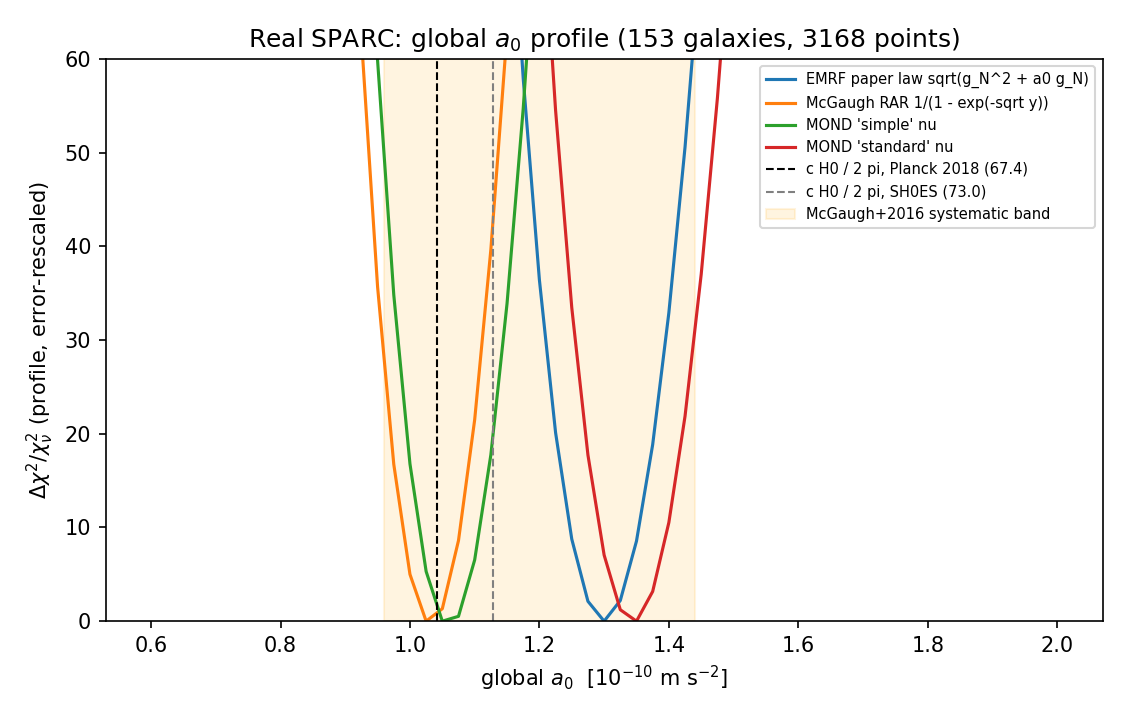
\includegraphics[width=0.85\textwidth]{figures/fig_real_sparc_a0_profile.png}
\caption{Profile of the global $a_0$ for the four laws (real SPARC data; $\Delta\chi^2$ rescaled by $\chi^2_\nu$). Dashed lines: $cH_0/2\pi$ for $H_0 = 67.4$ and $73.0$. Shaded: systematic band of Ref.~\cite{mcgaugh2016rar}.}
\label{fig:profile}
\end{figure}

\begin{figure}[h!]
\centering
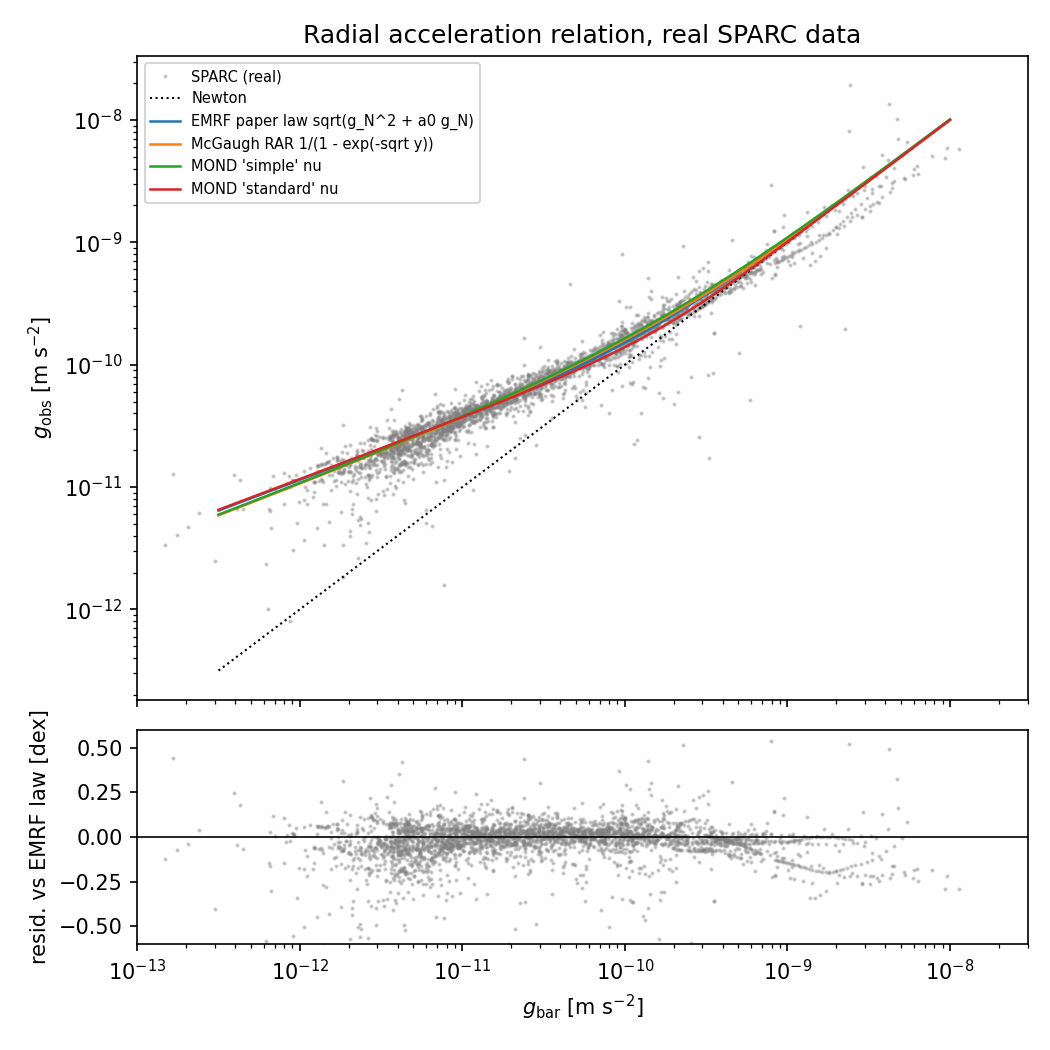
\includegraphics[width=0.7\textwidth]{figures/fig_real_sparc_rar.png}
\caption{Radial acceleration relation for the real SPARC sample, with the four laws at their best-fitting $a_0$. Lower panel: residuals with respect to the EMRF law.}
\label{fig:rar}
\end{figure}

The main findings (Table~\ref{tab:results}, Figs.~\ref{fig:profile}--\ref{fig:rar}) are:
\begin{enumerate}
\item \textbf{First pass: the horizon hypothesis is consistent with the data, but not confirmed} (superseded by the sharper test in Sec.~\ref{sec:marginalized}). For the RAR function the fitted $a_0$ spans $1.03$--$1.22$, which contains both values in Eq.~\eqref{eq:horizon}. The statistical uncertainty ($\sim$1\%) is much smaller than the $\Upsilon$ systematic ($\sim$20\%), in line with the published $\pm 0.24$ systematic \cite{mcgaugh2016rar}. A precision test would need independent stellar-mass and distance calibration.
\item \textbf{The earlier EMRF law is disfavoured.} $\sqrt{g_N^2 + a_0 g_N}$ fits worse than the RAR by $\Delta\mathrm{BIC} = +6{,}440$, its preferred $a_0$ (1.30--1.59) lies above $cH_0/2\pi$, and its $a_0/2$ Solar-System offset is excluded.
\item \textbf{Only the RAR function passes both tests} among those considered: it has the best galaxy fit and a negligible strong-field residual.
\item \textbf{Caveat on dark halos.} With distances and inclinations fixed, halo fits (two extra parameters per galaxy) are preferred by BIC. Ref.~\cite{li2018} shows that marginalizing over distance and inclination substantially improves single-$a_0$ fits, so this comparison isn't yet like-for-like. We don't claim that the data rule out, or require, dark matter.
\end{enumerate}

\section{Sharpened Test: Marginalizing Distance and Inclination}
\label{sec:marginalized}
Holding distances and inclinations at their catalogue values understates the uncertainties and biases $a_0$. Following Ref.~\cite{li2018}, each galaxy now carries three nuisance parameters with Gaussian priors: $\log\Upsilon_d$ ($\pm0.1$\,dex), a distance factor $f_D$ ($\sigma = e_D/D$) and the inclination ($\sigma = e_i$). Under $D \to f_D D$, $g_{\mathrm{bar}}$ is invariant while $g_{\mathrm{obs}} \propto 1/f_D$; under $i \to i'$, the observed velocities scale by $\sin i/\sin i'$. In the deep regime $a_0$ and the stellar mass scale are degenerate ($g \simeq \sqrt{a_0 g_{\mathrm{bar}}}$ with $g_{\mathrm{bar}} \propto \Upsilon$). We therefore decided before fitting to report the 66 \emph{gas-dominated} galaxies (gas fraction $> 0.5$; 966 points) separately, and to vary the prior centre $\Upsilon_0 \in \{0.4, 0.5, 0.6\}$. The estimator is unbiased on in-memory galaxies generated with wrong catalogue distances and inclinations. For the RAR function and the full sample it returns $a_0 = 1.234\times10^{-10}$\,m\,s$^{-2}$, matching the value of Ref.~\cite{li2018} obtained with this method ($1.20 \pm 0.02$).

\begin{table}[h!]
\centering
\small
\caption{Global $a_0$ ($10^{-10}$\,m\,s$^{-2}$) with distance, inclination and $\Upsilon_\star$ marginalized ($\Upsilon_0 = 0.5$). Errors combine the $\chi^2_\nu$-rescaled statistical error with half the range over $\Upsilon_0$. Pulls are relative to $cH_0/2\pi$ for $H_0 = 67.4$ / $73.0$ and to $c\sqrt{\Lambda/3}/2\pi = 0.863$.}
\label{tab:marginalized}
\begin{tabular}{lcccccc}
\toprule
& \multicolumn{3}{c}{All 153 galaxies ($\chi^2_\nu \approx 4.8$--$5.9$)} & \multicolumn{3}{c}{66 gas-dominated ($\chi^2_\nu \approx 2.6$)} \\
Law & $a_0$ & pull (67.4 / 73.0) & pull ($\Lambda$) & $a_0$ & pull (67.4 / 73.0) & pull ($\Lambda$) \\
\midrule
RAR & $1.234 \pm 0.048$ & $+4.0$ / $+2.2$ & $+7.8$ & $1.019 \pm 0.082$ & $-0.3$ / $-1.3$ & $+1.9$ \\
simple & $1.301 \pm 0.051$ & $+5.1$ / $+3.4$ & $+8.6$ & $1.023 \pm 0.081$ & $-0.2$ / $-1.3$ & $+2.0$ \\
EMRF $\sqrt{g_N^2 + a_0 g_N}$ & $1.583 \pm 0.061$ & $+8.8$ / $+7.4$ & $+11.8$ & $1.145 \pm 0.083$ & $+1.2$ / $+0.2$ & $+3.4$ \\
standard & $1.602 \pm 0.061$ & $+9.2$ / $+7.8$ & $+12.1$ & $1.144 \pm 0.087$ & $+1.2$ / $+0.2$ & $+3.2$ \\
\bottomrule
\end{tabular}
\end{table}

\begin{figure}[h!]
\centering
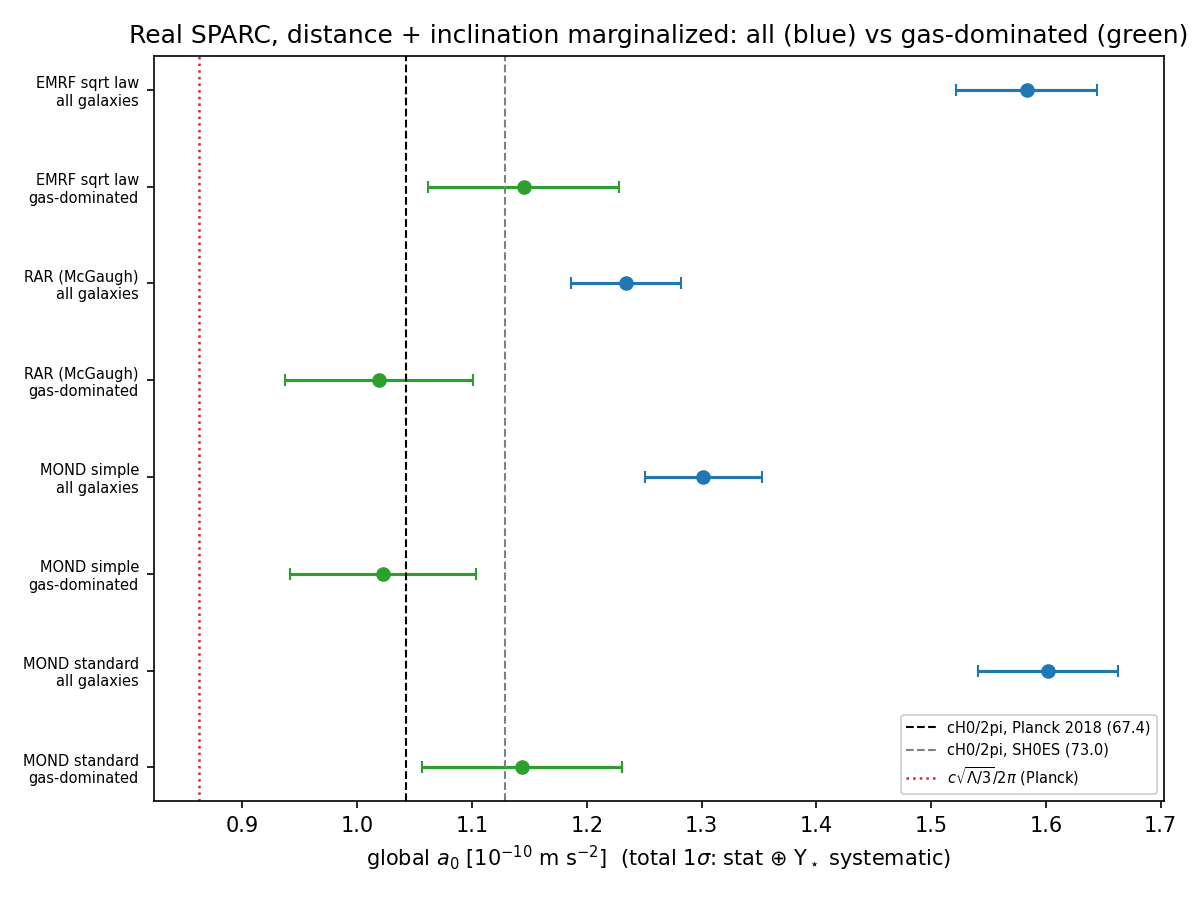
\includegraphics[width=0.8\textwidth]{figures/fig_real_sparc_a0_marginalized.png}
\caption{Global $a_0$ with distance, inclination and $\Upsilon_\star$ marginalized, for all galaxies (blue) and the gas-dominated subsample (green). Dashed lines: $cH_0/2\pi$ (Planck, SH0ES). Dotted red line: the $\Lambda$-tied variant.}
\label{fig:marginalized}
\end{figure}

The results (Table~\ref{tab:marginalized}, Fig.~\ref{fig:marginalized}) sharpen, and complicate, the conclusion of Sec.~\ref{sec:results}:
\begin{enumerate}
\item \textbf{Gas-dominated galaxies}, the subsample least sensitive to stellar masses and to the choice of law (spread $\pm0.06$ across laws), give $a_0 \approx 1.02$--$1.15$, consistent with $cH_0/2\pi$ within $1.3\sigma$ for both values of $H_0$ and every law.
\item \textbf{The full sample} gives a higher, law-dependent $a_0$ (spread $\pm0.18$). For the best-fitting RAR law it lies $4.0\sigma$ (Planck) and $2.2\sigma$ (SH0ES) above $cH_0/2\pi$.
\item \textbf{The two samples disagree} at about $2.3\sigma$ for the RAR law. Either the star-dominated galaxies carry unmodelled systematics (stellar-population gradients, bulges, non-circular motions), or a single $\nu(y)$ with a single $a_0$ doesn't describe both populations. Fits remain imperfect ($\chi^2_\nu > 1$). Section~\ref{sec:diagnostics} traces the disagreement to bulges.
\item \textbf{The $\Lambda$-tied variant} $a_0 = c\sqrt{\Lambda/3}/2\pi$, which would make $a_0$ constant in time, is disfavoured at $1.9$--$3.4\sigma$ even in the gas-dominated sample. The $H(z)$-tracking variant is disfavoured by high-redshift kinematics (Sec.~\ref{sec:other}). Each of the two natural readings of the horizon hypothesis therefore faces tension.
\item \textbf{The implied $H_0 = 2\pi a_0/c$} from the gas-dominated sample is $66 \pm 5$ (RAR) to $74 \pm 6$ (EMRF law)\,km\,s$^{-1}$\,Mpc$^{-1}$. That's too uncertain, and too dependent on the law, to inform the Hubble tension.
\end{enumerate}

\section{Diagnosing the Disagreement: Bulges, Not Gas}
\label{sec:diagnostics}
To find out where the gas/star disagreement comes from, we re-fitted the star-dominated galaxies after removing the places where stellar modelling, or the shape of the interpolating function, could bias $a_0$. The subsets were fixed before fitting: bulgeless galaxies only; ``deep'' points only ($g_{\mathrm{bar}} < 0.3\times1.2\times10^{-10}$\,m\,s$^{-2}$ at $\Upsilon = 0.5$, where every law reduces to $\sqrt{a_0 g_{\mathrm{bar}}}$); and locally gas-dominated points. Because removing bulges moved $a_0$ strongly, we then also fitted the complementary bulge galaxies. That step was added after seeing the first result, and we label it post hoc. All fits use the RAR law with distance, inclination and $\Upsilon_\star$ marginalized as in Sec.~\ref{sec:marginalized}.

\begin{table}[h!]
\centering
\small
\caption{Global $a_0$ ($10^{-10}$\,m\,s$^{-2}$) for diagnostic subsets of the real SPARC sample (RAR law). Pulls are relative to $cH_0/2\pi$ for $H_0 = 67.4$ / $73.0$.}
\label{tab:diagnostics}
\begin{tabular}{llrrccc}
\toprule
& Subset & Gal. & Pts & $a_0$ & $\chi^2_\nu$ & pull (67.4 / 73.0) \\
\midrule
A & gas-dominated (reference) & 66 & 966 & $1.019 \pm 0.080$ & 2.6 & $-0.3$ / $-1.4$ \\
B & star-dominated, all points & 87 & 2202 & $1.276 \pm 0.062$ & 5.7 & $+3.8$ / $+2.4$ \\
C & star-dominated, bulgeless & 56 & 1070 & $0.894 \pm 0.050$ & 4.4 & $-3.0$ / $-4.7$ \\
D & star-dominated, deep points & 75 & 919 & $1.162 \pm 0.075$ & 2.7 & $+1.6$ / $+0.4$ \\
E & star-dominated, local-gas points & 6 & 50 & $0.915 \pm 0.122$ & 0.6 & $-1.0$ / $-1.8$ \\
F & star-dominated, bulgeless, deep & 50 & 614 & $0.840 \pm 0.065$ & 1.8 & $-3.1$ / $-4.4$ \\
G & all galaxies, deep points & 141 & 1859 & $1.098 \pm 0.062$ & 2.6 & $+0.9$ / $-0.5$ \\
H & star-dominated, with bulge (post hoc) & 31 & 1132 & $1.910 \pm 0.181$ & 6.6 & $+4.8$ / $+4.3$ \\
I & with bulge, deep points (post hoc) & 25 & 305 & $1.616 \pm 0.149$ & 3.9 & $+3.9$ / $+3.3$ \\
\bottomrule
\end{tabular}
\end{table}

\begin{figure}[h!]
\centering
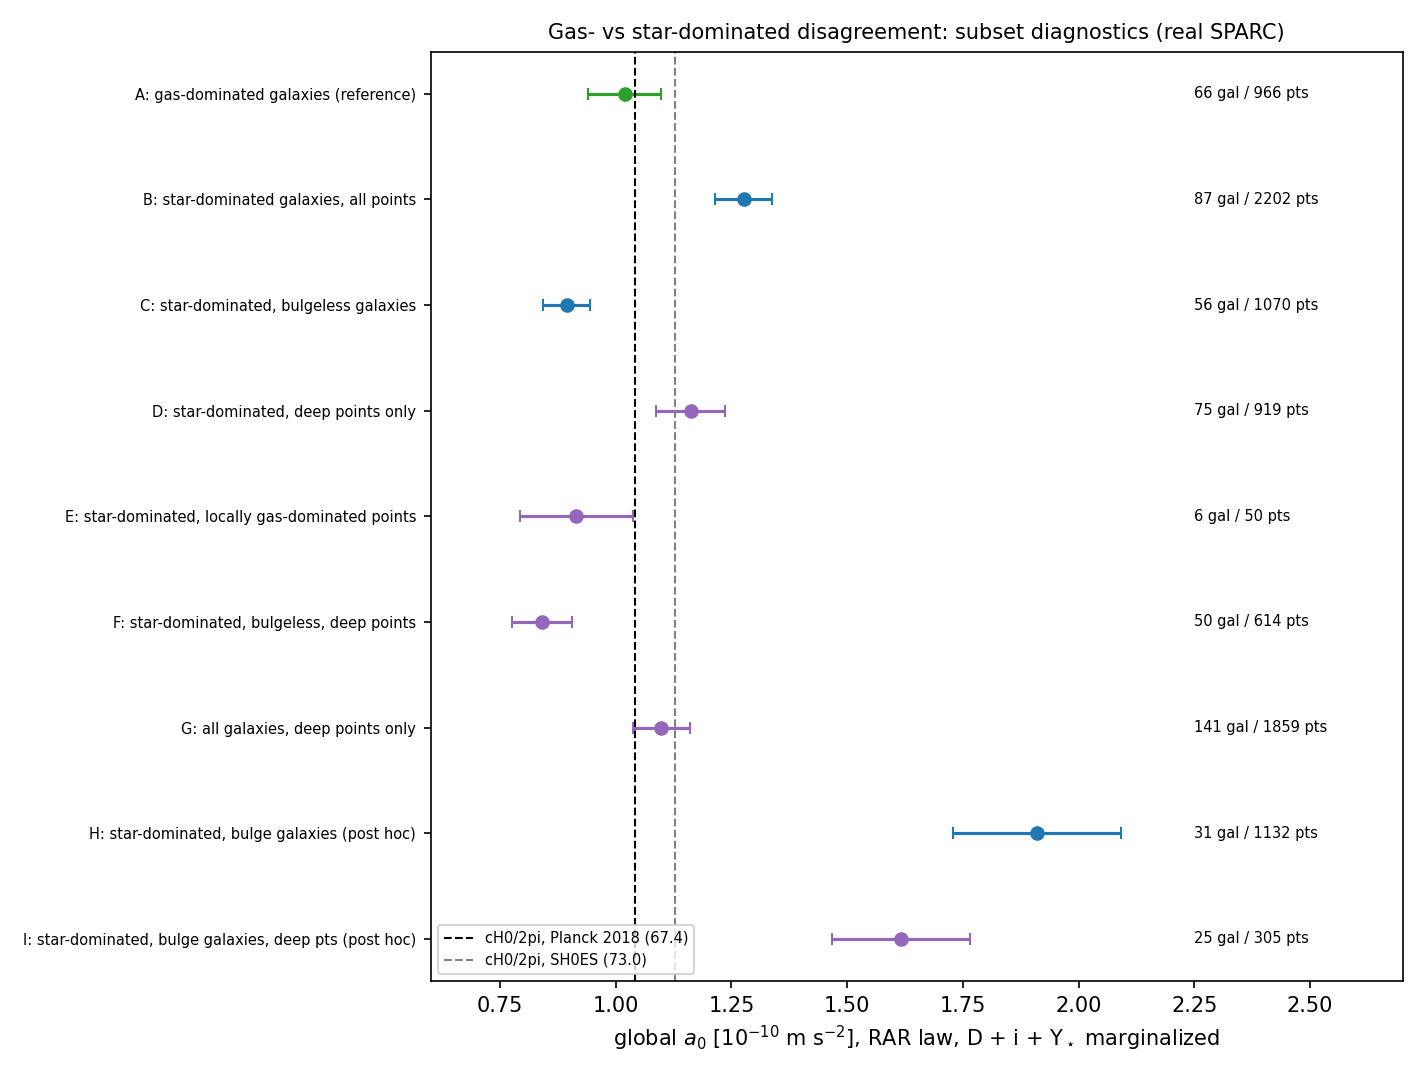
\includegraphics[width=0.85\textwidth]{figures/fig_real_sparc_tension_diagnostics.png}
\caption{Global $a_0$ for the diagnostic subsets of Table~\ref{tab:diagnostics}. Purple: deep or locally gas-dominated points only.}
\label{fig:diagnostics}
\end{figure}

The findings are:
\begin{enumerate}
\item \textbf{The disagreement is driven by galaxies with bulges.} The 31 star-dominated bulge galaxies prefer $a_0 = 1.91 \pm 0.18$, $5.4\sigma$ above the 56 bulgeless star-dominated galaxies ($0.894 \pm 0.050$; independent samples). The gap persists in deep points alone ($4.8\sigma$), so it isn't confined to the inner, bulge-dominated radii. Bulge galaxies also fit worst ($\chi^2_\nu = 6.6$).
\item \textbf{A single universal $a_0$ can't fit both populations with the current mass models.} Either the bulge mass models are wrong (in the deep regime $a_0$ and the baryonic mass are degenerate, so underestimated bulge masses or $\Upsilon_{\mathrm{bulge}}$ would mimic a larger $a_0$), or $a_0$ isn't universal. The second option would undermine MOND-type phenomenology and the horizon hypothesis alike. Distinguishing the two needs independent bulge mass estimates.
\item \textbf{Once bulges are removed, gas- and star-dominated galaxies agree} ($1.3\sigma$). Their inverse-variance combination (post hoc) is $a_0 = 0.930 \pm 0.042$, which lies \emph{below} $cH_0/2\pi$ ($-2.7\sigma$ Planck, $-4.7\sigma$ SH0ES) and above the $\Lambda$-tied value ($+1.6\sigma$).
\item \textbf{In the deep regime the law dependence collapses:} for subset D the four laws give $1.06$--$1.20$ (half-range $0.07$, versus $0.18$ for all points). Deep points of all galaxies give $1.098 \pm 0.062$, consistent with $cH_0/2\pi$ ($+0.9\sigma$ / $-0.5\sigma$), but that sample still includes bulge galaxies.
\end{enumerate}
Different defensible galaxy selections thus give $a_0$ between $0.84$ and $1.28$ (excluding the bulge-only subsets), a spread much larger than the formal errors. The determination of $a_0$ from current SPARC mass models is limited by systematics at the $\pm15$--$20\%$ level, in line with the $\pm0.24$ systematic of Ref.~\cite{mcgaugh2016rar}. At that level the data can't decide whether $a_0 = cH_0/2\pi$, and this test can't settle the hypothesis.

\section{Bulge Mass-to-Light Test}
\label{sec:bulge}
Is the bulge discrepancy a mass-model problem or a sign that $a_0$ isn't universal? We fixed this test before running it, for the 31 star-dominated bulge galaxies. Test~1 scales all bulge masses ($\Upsilon_b = r\,\Upsilon_d$, standard $r = 1.4$) and profiles $a_0$. Test~2 fixes $a_0$ (at $0.930$ and at $cH_0/2\pi = 1.042$) and frees each galaxy's $\Upsilon_b$. The plausibility bounds were set in advance relative to the stellar-population expectation $\Upsilon_b \approx 0.7$: up to $1.0$ plausible, $1.0$--$1.4$ stretched, above $1.4$ implausible.

The first run showed that we'd assumed the wrong direction: \emph{heavier} bulges \emph{raise} the fitted $a_0$. The bulge mass is pinned by the inner rotation curve, and a heavier bulge forces a lighter disk, so the outer curve needs more boost. We therefore added three things post hoc: lighter ratios ($r = 0.25$--$0.75$); symmetric lower bounds ($0.5$ plausible, $0.35$ stretched); and Test~3, which profiles $a_0$ with every $\Upsilon_b$ free.

\begin{figure}[h!]
\centering
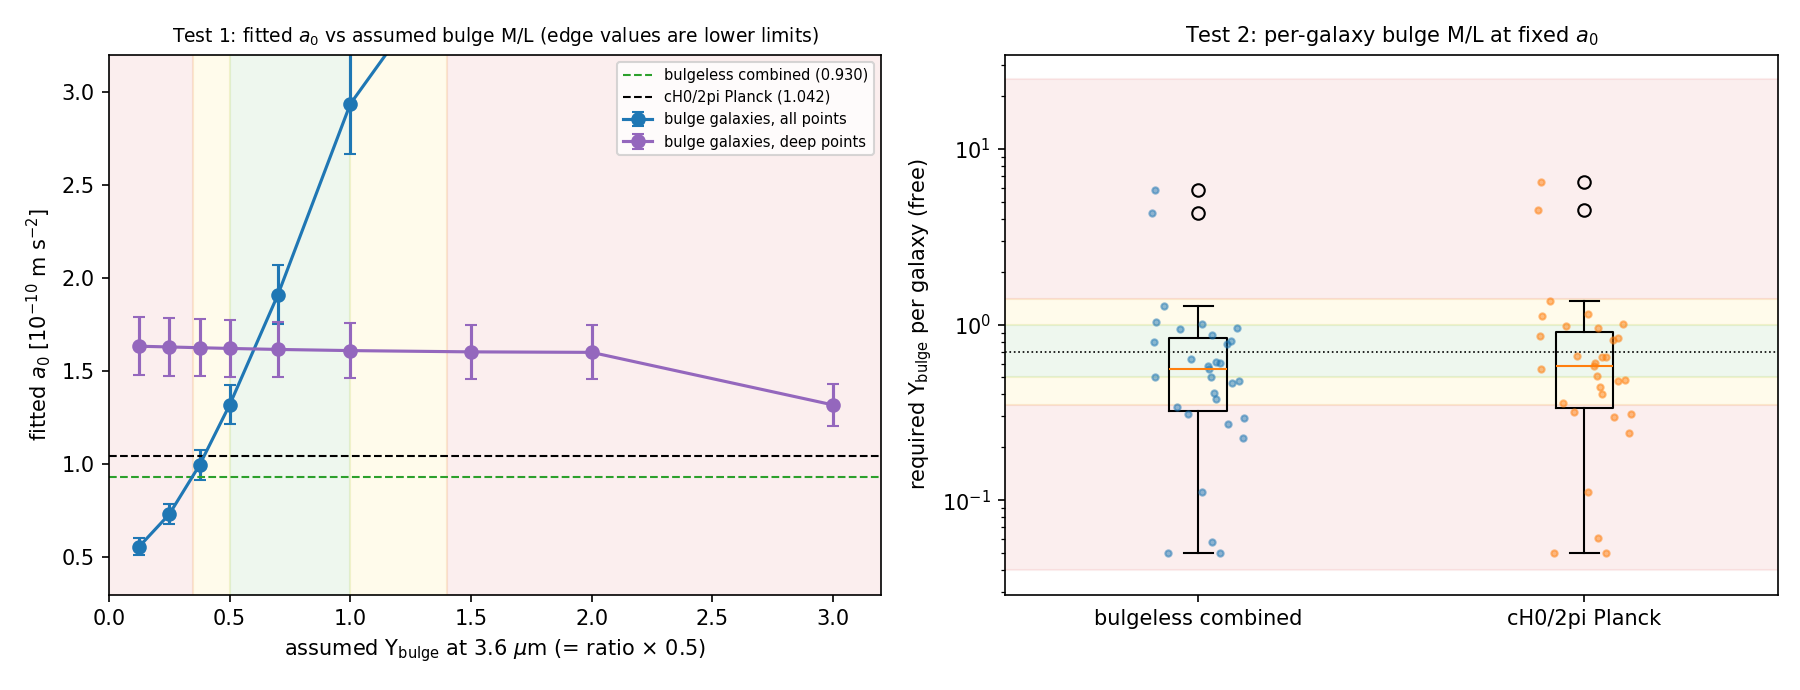
\includegraphics[width=\textwidth]{figures/fig_real_sparc_bulge_test.png}
\caption{Left: fitted $a_0$ for the 31 star-dominated bulge galaxies versus the assumed bulge mass-to-light ratio (all points, blue; deep points, purple). Shading marks plausible (green), stretched (yellow) and implausible (red) values. Right: per-galaxy bulge mass-to-light ratio required at fixed $a_0$.}
\label{fig:bulge}
\end{figure}

The results (Fig.~\ref{fig:bulge}) are:
\begin{enumerate}
\item \textbf{All points:} $a_0$ falls to the bulgeless value ($0.930$) only if $\Upsilon_b \approx 0.34$, and to $cH_0/2\pi$ only if $\Upsilon_b \approx 0.39$. That's half the expected bulge mass, and the fit worsens ($\chi^2_\nu$ rises from $6.4$ to $7$--$9$).
\item \textbf{Deep points:} $a_0 \approx 1.60$--$1.63$ for \emph{every} assumed $\Upsilon_b$ from $0.12$ to $2.0$, and $1.61$--$1.64$ for disk priors $\Upsilon_0 = 0.4$--$0.6$. No plausible stellar mass-to-light ratio brings the outer, deep regime of these galaxies to $\approx 1$.
\item \textbf{Every bulge free (Test 3):} $a_0 = 1.28 \pm 0.13$. The bulgeless value ($0.930$) is disfavoured at $\Delta\chi^2 \approx 10.7$ (about $3.3\sigma$) and $cH_0/2\pi$ at $\Delta\chi^2 \approx 4.2$ (about $2\sigma$). Per galaxy, the required $\Upsilon_b$ has a median of $0.56$--$0.58$ but scatters widely ($16$--$84\%$: $0.26$--$1.0$); about a third of galaxies fall in the implausible range.
\end{enumerate}
Stellar mass-to-light mis-modelling therefore isn't sufficient to explain why bulge galaxies prefer a larger $a_0$. What remains is either other systematics specific to these massive, early-type disks (distance errors beyond the catalogued ones, non-circular motions, warps or outer-disk inclination changes), or a genuinely non-universal acceleration scale. Universality of $a_0$ is contested in the literature \cite{rodrigues2018,mcgaugh2018reply,kroupa2018reply}. Our data can't decide between these options. Either way, a single universal $a_0 = cH_0/2\pi$ does \emph{not} describe these 31 galaxies with standard mass models.

\section{Status of Other Regimes and Prior Work}
\label{sec:other}
\textbf{Sagittarius~A* S-stars.} EMRF is \emph{required} to reduce to General Relativity when $a \gg a_0$. At the pericentres of S2 or S301 ($g \sim 1$--$100$\,m\,s$^{-2}$) every law in Sec.~\ref{sec:laws} differs from Newton by $\lesssim a_0$. These orbits therefore can't discriminate EMRF from GR, beyond confirming GR itself \cite{gravity2018,gravity2020,gravity2022,gravity2026s301}. The earlier claim that EMRF ``derives'' the Schwarzschild metric is withdrawn.

\textbf{Redshift evolution.} If $a_0 = cH(z)/2\pi$, then $a_0$ grows by a factor $\simeq 3$ by $z = 2$. Rotation curves at $z \approx 1$--2.5 show baryon-dominated inner disks with \emph{lower} dark-matter fractions at higher redshift \cite{genzel2017,shachar2023}. That runs opposite to the trend expected from a growing $a_0$, so strong evolution is disfavoured. A real-data test is future work.

\textbf{Wide binaries, clusters, lensing, CMB.} Gaia wide-binary analyses disagree \cite{chae2023,banik2024}, and careful treatments of triple-star contamination favour Newtonian dynamics \cite{banik2024}. MOND-type laws leave residual missing mass in clusters, including the Bullet Cluster \cite{clowe2006,angus2007}. Lensing and the CMB need a relativistic completion \cite{skordis2021}. EMRF currently makes no calculation in these regimes. Verlinde's entropic formula, a close relative of the horizon idea, was found inconsistent with the RAR of individual galaxies \cite{lelli2017verlinde}.

\section{Conclusion}
\label{sec:conclusion}
Tested against real data, EMRF's horizon hypothesis $a_0 = cH_0/2\pi$ is neither confirmed nor excluded. Gas-dominated galaxies, the cleanest probe, agree with it. The full sample, which reproduces the literature value $a_0 \approx 1.2\times10^{-10}$, sits $2$--$4\sigma$ above it. That excess is driven by galaxies with bulges, and a dedicated test shows no plausible bulge or disk mass-to-light ratio removes it in their outer, deep regime. Bulgeless galaxies instead sit somewhat below $cH_0/2\pi$. A single universal $a_0 = cH_0/2\pi$ doesn't describe the bulge galaxies with standard mass models. Whether that reflects unmodelled systematics or a non-universal $a_0$ is open, and with current data $a_0$ is uncertain by $\pm15$--$20\%$, too much to decide the question. Neither natural reading of the hypothesis is free of tension: an $H(z)$-tracking $a_0$ runs against high-redshift kinematics, and a $\Lambda$-tied $a_0$ is too small. The specific law used in earlier EMRF drafts is disfavoured by both galaxies and the Solar System. The framework's open tasks are:
(1) test the remaining explanations for the bulge-galaxy discrepancy, namely independent distances (e.g.\ TRGB or Cepheid), resolved two-dimensional kinematics for non-circular motions and warps, and independent stellar masses, or else accept a non-universal $a_0$;
(2) derive an RAR-like interpolating function from an action with a non-canonical kinetic term;
(3) test redshift evolution against published high-$z$ kinematics;
(4) address lensing, clusters and the CMB with a relativistic completion.

\section*{Reproducibility and data availability}
\label{sec:repro}
All code is at \url{https://github.com/kirklasalle/SpaceEntropyCompression}. \texttt{python emergent\_matter\_model/sparc\_real\_analysis.py} downloads SPARC \cite{lelli2016sparc}, verifies and records checksums, and regenerates Table~\ref{tab:results} and Figs.~\ref{fig:profile}--\ref{fig:rar} (results file \texttt{results/sparc\_real\_analysis.json}). \texttt{python emergent\_matter\_model/sparc\_marginalized\_a0.py} regenerates Table~\ref{tab:marginalized} and Fig.~\ref{fig:marginalized} (about 12 minutes; \texttt{results/sparc\_marginalized\_a0.json}). \texttt{python emergent\_matter\_model/sparc\_tension\_diagnostics.py} regenerates Table~\ref{tab:diagnostics} and Fig.~\ref{fig:diagnostics} (about 20 minutes; \texttt{results/sparc\_tension\_diagnostics.json}). \texttt{python emergent\_matter\_model/sparc\_bulge\_test.py} regenerates Fig.~\ref{fig:bulge} (about 15 minutes; \texttt{results/sparc\_bulge\_test.json}). The audit that motivated this revision, with every hand calculation written out, is in \texttt{docs/SHOW\_YOUR\_WORK.md}, and it is reproduced by \texttt{tools/show\_your\_work\_audit.py}.

\section*{Acknowledgments}
The author thanks the SPARC team for making their data public. Software development and the audit were assisted by AI coding tools. All numerical claims were independently recomputed from public data, and the author takes responsibility for the content.

\bibliographystyle{unsrt}
\bibliography{references}

\end{document}
